\newpage
\begin{center}
  \textbf{\large 3. РАЗРАБОТКА ПРОГРАМНОГО ПРОДУКТА}
\end{center}
\refstepcounter{chapter}
\addcontentsline{toc}{chapter}{3. РАЗРАБОТКА ПРОГРАМНОГО ПРОДУКТА}

\section{Выбор инструментов разработки}
Первый этап процесса разработки заключался в выборе инструментов, которые будут использоваться в процессе разработки.

\textbf{IDE IntelliJ Idea} была выбрана в качестве рабочей среды для разработки сервисов.
Она предоставляет широкий набор функций и инструментов для разработки на языке Kotlin.

В качестве тестовой базы данных было решено использовать Docker-образ MongoDB. 
Docker-контейнер позволяет легко развернуть и настроить локальное окружение MongoDB, обеспечивая изолированную и портативную среду разработки. 

\textbf{Visual Studio Code} была выбрана в качестве рабочей среды для разработки мобильного приложения.
Она предоставляет широкий набор функций и инструментов для разработки на языке Dart.

\section{Процесс разработки сервисов}
\subsection{Общий модуль (core)}
Уже перед началом разработки было понятно, что сервисы будут иметь много схожей логики (модели данных, работа с БД, валидация данных, обработка ошибок, логирование и т.д.).
Поэтому для соблюдения принципа DRY 
\footnote{Don’t repeat yourself (DRY; с англ. — «не повторяйся») — это принцип разработки программного обеспечения, нацеленный на снижение повторения информации различного рода, особенно в системах со множеством слоёв абстрагирования.} 
было решено выделить общую часть в отдельный модуль, который будет подключаться к каждому сервису как зависимость. Данный модуль был назван \textbf{core}.
Структурная схема модулей и микросервисов представлена на рисунке \ref{fig:schemes:services}.

\begin{figure}
  \centering
  \includegraphics[width=0.8\linewidth]{images/schemes/services.png}
  \caption{Схема модулей серверной части. Линии показывают направление зависимостей.}
  \label{fig:schemes:services}
\end{figure}

Core модуль инкапсулирует в себе несколько функций: работа с данными, конфигурация, DI
\footnote{Dependency injection (DI) или внедрение зависимостей представляет механизм, который позволяет сделать компоненты программы слабосвязанными, 
а всю программу в целом более гибкой, более адаптируемой и расширяемой.
}, и предоставление общих внешних зависимостей.

Работа с данными включает себя описание моделей данных и репозиториев
\footnote{Репозиторий - это слой абстракции, инкапсулирующий в себе всё, что относится к способу хранения данных. 
Назначение: Разделение бизнес-логики от деталей реализации слоя доступа к данным.}
для работы с БД. Код моделей доступен по ссылке 6.1.\ref{code:models}. Код репозиториев доступен по ссылке 6.1.\ref{code:repo}.

Конфигурация представляет собой класс, который содержит в себе порт, 
адрес БД, настройки email-сервера, настройки S3 хранилища и т.д.
Конфигурация переиспользуется в каждом сервисе.
Код конфигурации доступен по ссылке 6.1.\ref{code:config}.

DI реализован с помощью библиотеки Koin. Core модуль предоставляет общий DI контейнер, 
с уже зарегистрированными фабриками
\footnote{Фабрика – это порождающий паттерн проектирования, который позволяет создавать обьекты, не привязываясь к конкретным реализациям.}
и одиночками 
\footnote{Одиночка (Singleton, Синглтон) - порождающий паттерн, который гарантирует, что для определенного класса будет создан только один объект.}
для всех общих зависимостей. Далее каждый сервис может получить этот контейнер, 
зарегистрировать в нем свои зависимости, не используя конкретные реализации.
Код DI контейнера доступен по ссылке 6.1.\ref{code:di}.

Общие внешние зависимости представляют собой библиотеки, которые используются в каждом сервисе. 
Core модуль предоставляет следующие зависимости:
\begin{enumerate}
  \item graphql-kotlin-federation -- Библиотека для разметки схемы GraphQL.
  \item kmongo -- Библиотека для работы с MongoDB.
  \item koin -- Библиотека для реализации DI.
  \item logback -- Библиотека для логирования.
\end{enumerate}
Исходный код общих внешних зависимостей доступен по ссылке 6.1.\ref{code:gradle}.

Общие утилиты представляют собой классы, которые содержат вспомогательные функции. В контексте данной АИС это:
\begin{enumerate}
  \item Рассчет расписания на определенный период времени для заданного списка предметов.
  \item Рассчет хеш суммы для набора параметров поиска расписания.
\end{enumerate}
Исходный код общих утилит доступен по ссылке 6.1.\ref{code:utils}.

\subsection{Сервис API (backend)}

Сервис backend предназначен для обеспечения доступа мобильного приложения и других сервисов
к данным расписания, хранящимся в базе данных. Он написан на языке программирования Kotlin с использованием фреймворка Spring и базы данных Mongo DB.
Сервис спроектирован по паттерну “Чистая архитектура”.

В ходе разработки были созданы следующие публичные методы:
\begin{enumerate}
\item \texttt{findGroups} позволяет находить группы по заданным параметрам (например, по названию или описанию). 
Это может быть полезно для пользователей, которые ищут конкретную группу или группы, соответствующие определенным критериям.
\item \texttt{groupById} позволяет получать информацию о группе по ее идентификатору. 
Этот метод может быть полезен для пользователей, которые знают идентификатор интересующей их группы и хотят получить о ней подробную информацию.
\item \texttt{findDisciplines} позволяет находит предметы по названию. 
Это может быть полезно для пользователей, которые ищут информацию о конкретном предмете или хотят найти все предметы, соответствующие определенным критериям.
\item \texttt{disciplineById} позволяет получать информацию о предмете по его идентификатору. 
Это может быть полезно для пользователей, которые знают идентификатор интересующего их предмета и хотят получить о нем подробную информацию.
\item \texttt{findTeachers} позволяет находить преподавателей по заданным параметрам (например, по имени или фамилии). 
Это может быть полезно для пользователей, которые ищут конкретного преподавателя или хотят найти всех преподавателей, соответствующих определенным критериям.
\item \texttt{teacherById} позволяет получать информацию о преподавателе по его идентификатору. 
Этот метод может быть полезен для пользователей, которые знают идентификатор интересующего их преподавателя и хотят получить о нем подробную информацию.
\item \texttt{findRooms} позволяет находить аудитории по заданным параметрам (например, по номеру или корпусу). 
Это может быть полезно для пользователей, которые ищут конкретную аудиторию или хотят найти все аудитории, соответствующие определенным критериям.
\item \texttt{roomById} позволяет получать информацию о конкретной аудитории по ее идентификатору. 
Это может быть полезно для пользователей, которые знают идентификатор интересующей их аудитории и хотят получить о ней подробную информацию.
\item \texttt{findRegularLessons} позволяет находить расписание занятий по заданным параметрам.
Это может быть полезно для пользователей, которые ищут занятия по определенному предмету, учителю или аудитории, или хотят найти все занятия, соответствующие определенным критериям.
\item \texttt{regularLessonById} позволяет получать информацию о конкретном занятии по его идентификатору. 
Это может быть полезно для пользователей, которые знают идентификатор интересующего их занятия и хотят получить о нем подробную информацию.
\item \texttt{findDayLessons} позволяет получить расписание занятий по заданным фильтрам (группа, аудитория, преподаватель, предмет) на конкретные даты.
\item \texttt{findDayLessonsForNextDays} позволяет получить расписание занятий на ближайшие дни. 
Пользователи могут выбрать количество дней, на которые они хотят получить расписание занятий, и фильтры (группа, аудитория, преподаватель, предмет).
\item \texttt{calendarByFilter} возвращает URL-адрес ICS-файла с расписанием занятий, отфильтрованным по заданным параметрам. Этот URL-адрес можно интегрировать в любое приложение календаря для импорта расписания занятий в календарь.
\end{enumerate}

Вся техническая документация сервиса GraphQL API, доступна по ссылке:
\url{https://mtuci.stereobreeze.ru/playground}.
Там располагается расширенное описание сервиса, описания всех публичных методов и их параметров, а также примеры запросов и ответов.
Пример документации сервиса представлен на рисунке \ref{fig:back:doc}.

\begin{figure}
  \centering
  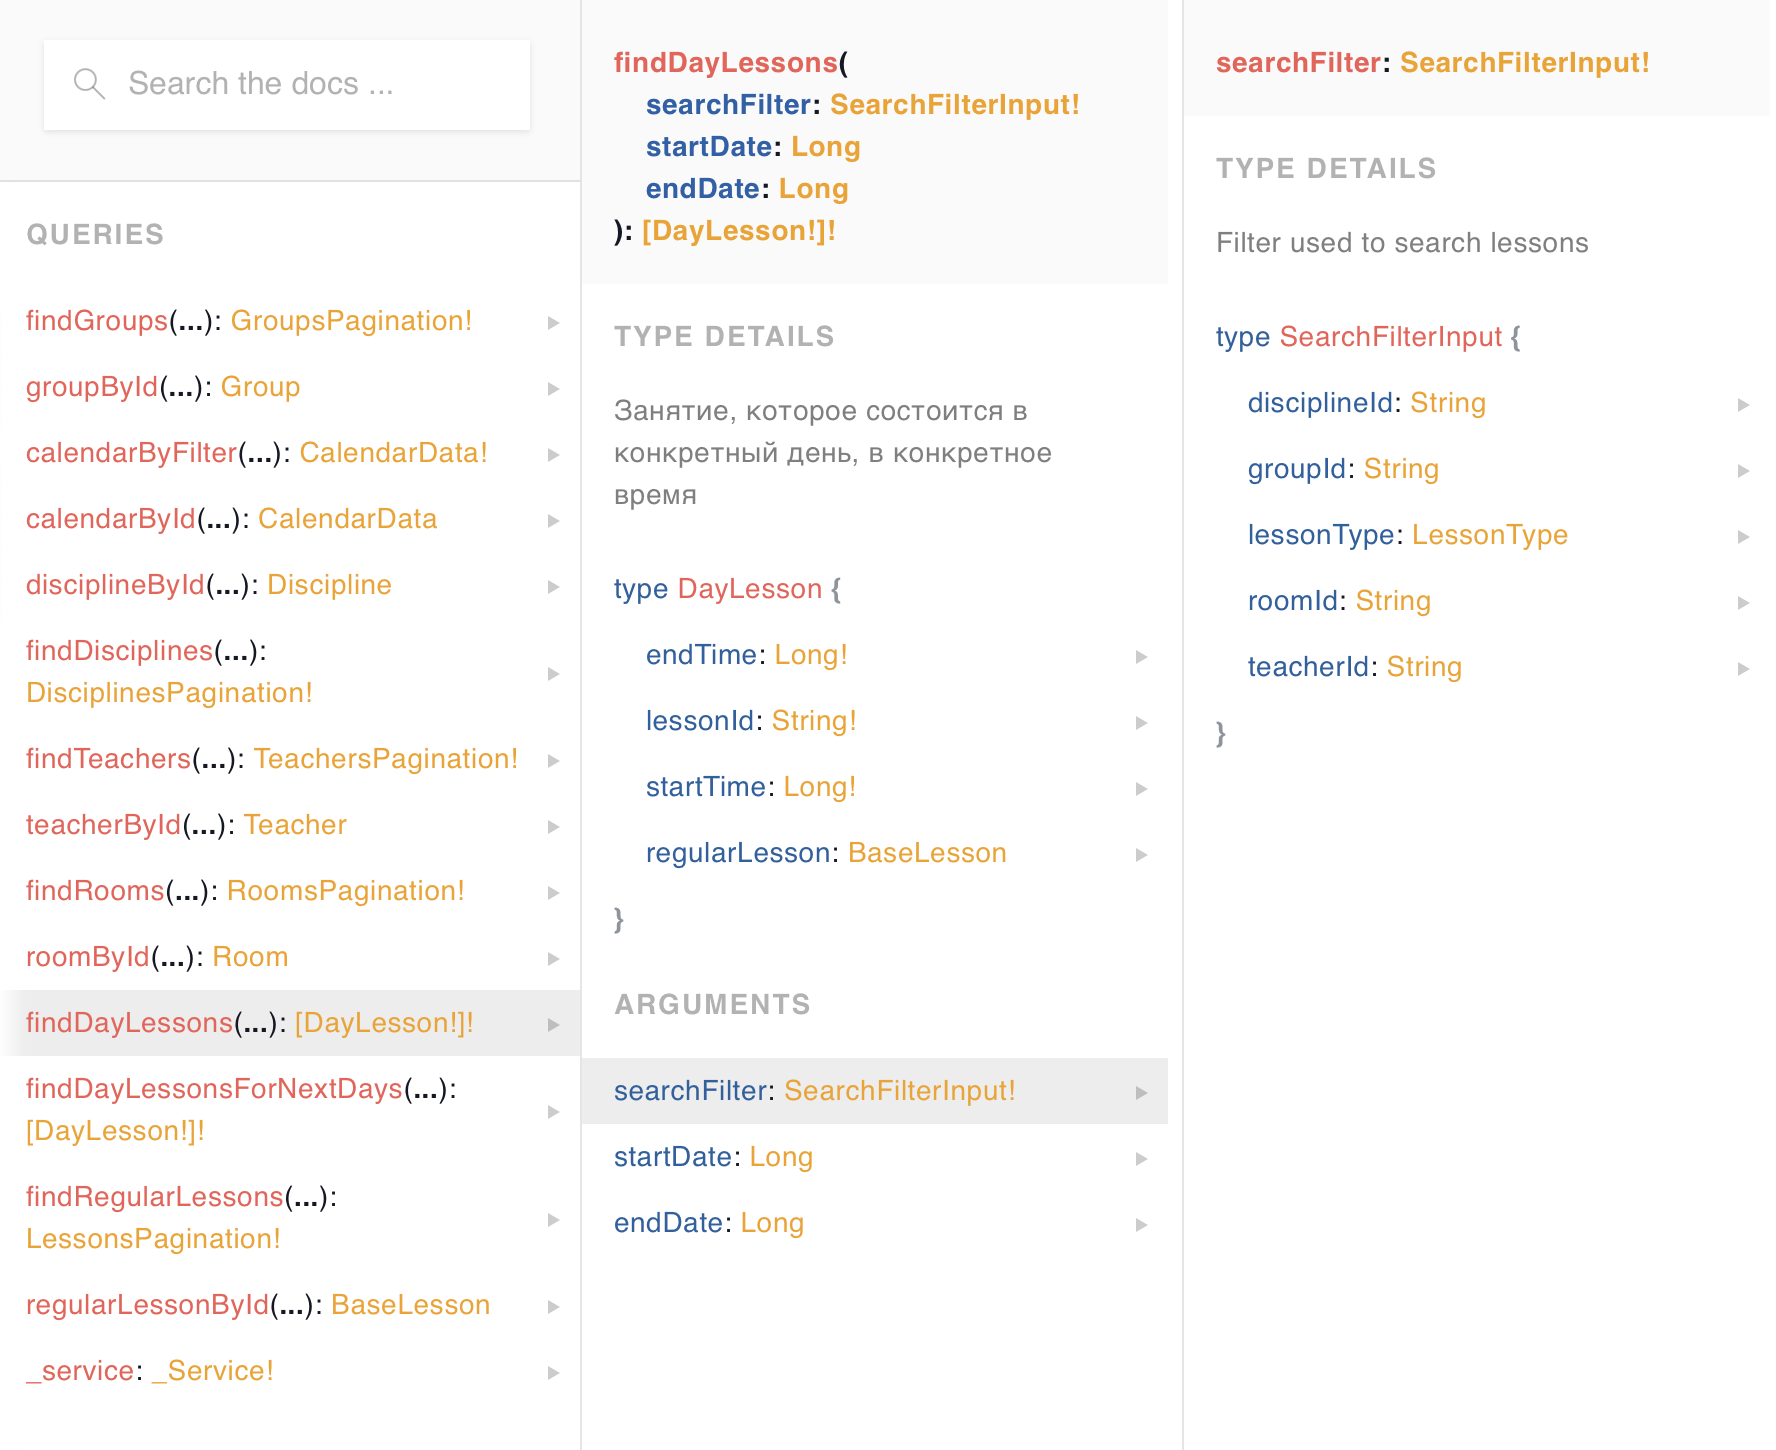
\includegraphics[width=0.8\linewidth]{images/back/doc.png}
  \caption{Пример документации сервиса GraphQL API}
  \label{fig:back:doc}
\end{figure}

На данный момент сервис активен, и доступен по публичному адресу \url{https://mtuci.stereobreeze.ru/playground}.
Исходный код сервиса доступен по ссылке: \url{https://github.com/alexsvdk/mtuci_rasp_back/tree/master/backend}.

\break
\subsection{Сервис парсинга расписания занятий (parser)}
Сервис парсига расписания предназначен для извлечения данных расписания из exel 
файла в формате \texttt{*.xlsx} и сохранения их в базу данных.

% todo рассказать подробнее хз о чем

На данный момент сервис активен, и принимает данные на почтом ящик a.s.shvedchikov@mtuci.ru. 
Исходный код сервиса расположен на доступен по ссылке \url{https://github.com/alexsvdk/mtuci_rasp_back/tree/master/parser}.
123123

\subsection{Сервис интеграции календаря (ics\textunderscore backend)}
Микросервис ICS API предназначен для генерации ICS-файлов с расписанием занятий 
и экзаменов по заданным фильтрам. Пользователи могут выбрать группу, аудиторию, 
преподавателя, предмет и даты, на которые они хотят получить расписание занятий и экзаменов. 
После выбора фильтров, микросервис генерирует ICS-файл, который можно импортировать в календарь, 
такой как Google Calendar или Microsoft Outlook. Кроме того, микросервис предоставляет возможность 
подписаться на календарь по URL. Это позволяет пользователям получать обновленное расписание занятий 
и экзаменов в своем календаре без необходимости ручного импорта файла.

Алгоримт работы микросервиса:
\begin{enumerate}
\item Пользователь узнает URL ICS файла календаря через метод GraphQL \texttt{calendarByFilter}.
\item При первоначальном обращении по URL микросервис получает фильтры из URL и данные о занятиях и экзаменах из будет, соответствующих заданным фильтрам. 
Затем микросервис генерирует ICS-файл на основе полученных данных и возвращает его пользователю и сохраняет в файловае распределенное хранилище S3.
\item При последующих обращениях по URL микросервис проверяет актуальность уже сгенерированного файла при помощи механизма ведения ревизий, 
и если файл все еще актуальный - возвращает HTTP код переадресации на ICS из файлового хранилища.
\end{enumerate}

При создании событий в ICS файле, микросервис указывает следующие данные:
\begin{enumerate}
  \item Название события, например: Лекция по математике.
  \item Место проведения события, например: аудитория 101.
  \item Дату и время начала и окончания события.
  \item Повторяемость события, например: каждую неделю.
  \item Тип занятия: лекция, практика, лабораторная работа, экзамен.
  \item Информация о преподавателе, например: ФИО, email, должность.
\end{enumerate}
Пример отображения сгенерированных ICS событий в пользовательском календаре представлен на рисунке \ref{fig:back:ics}.

\begin{figure}
  \centering
  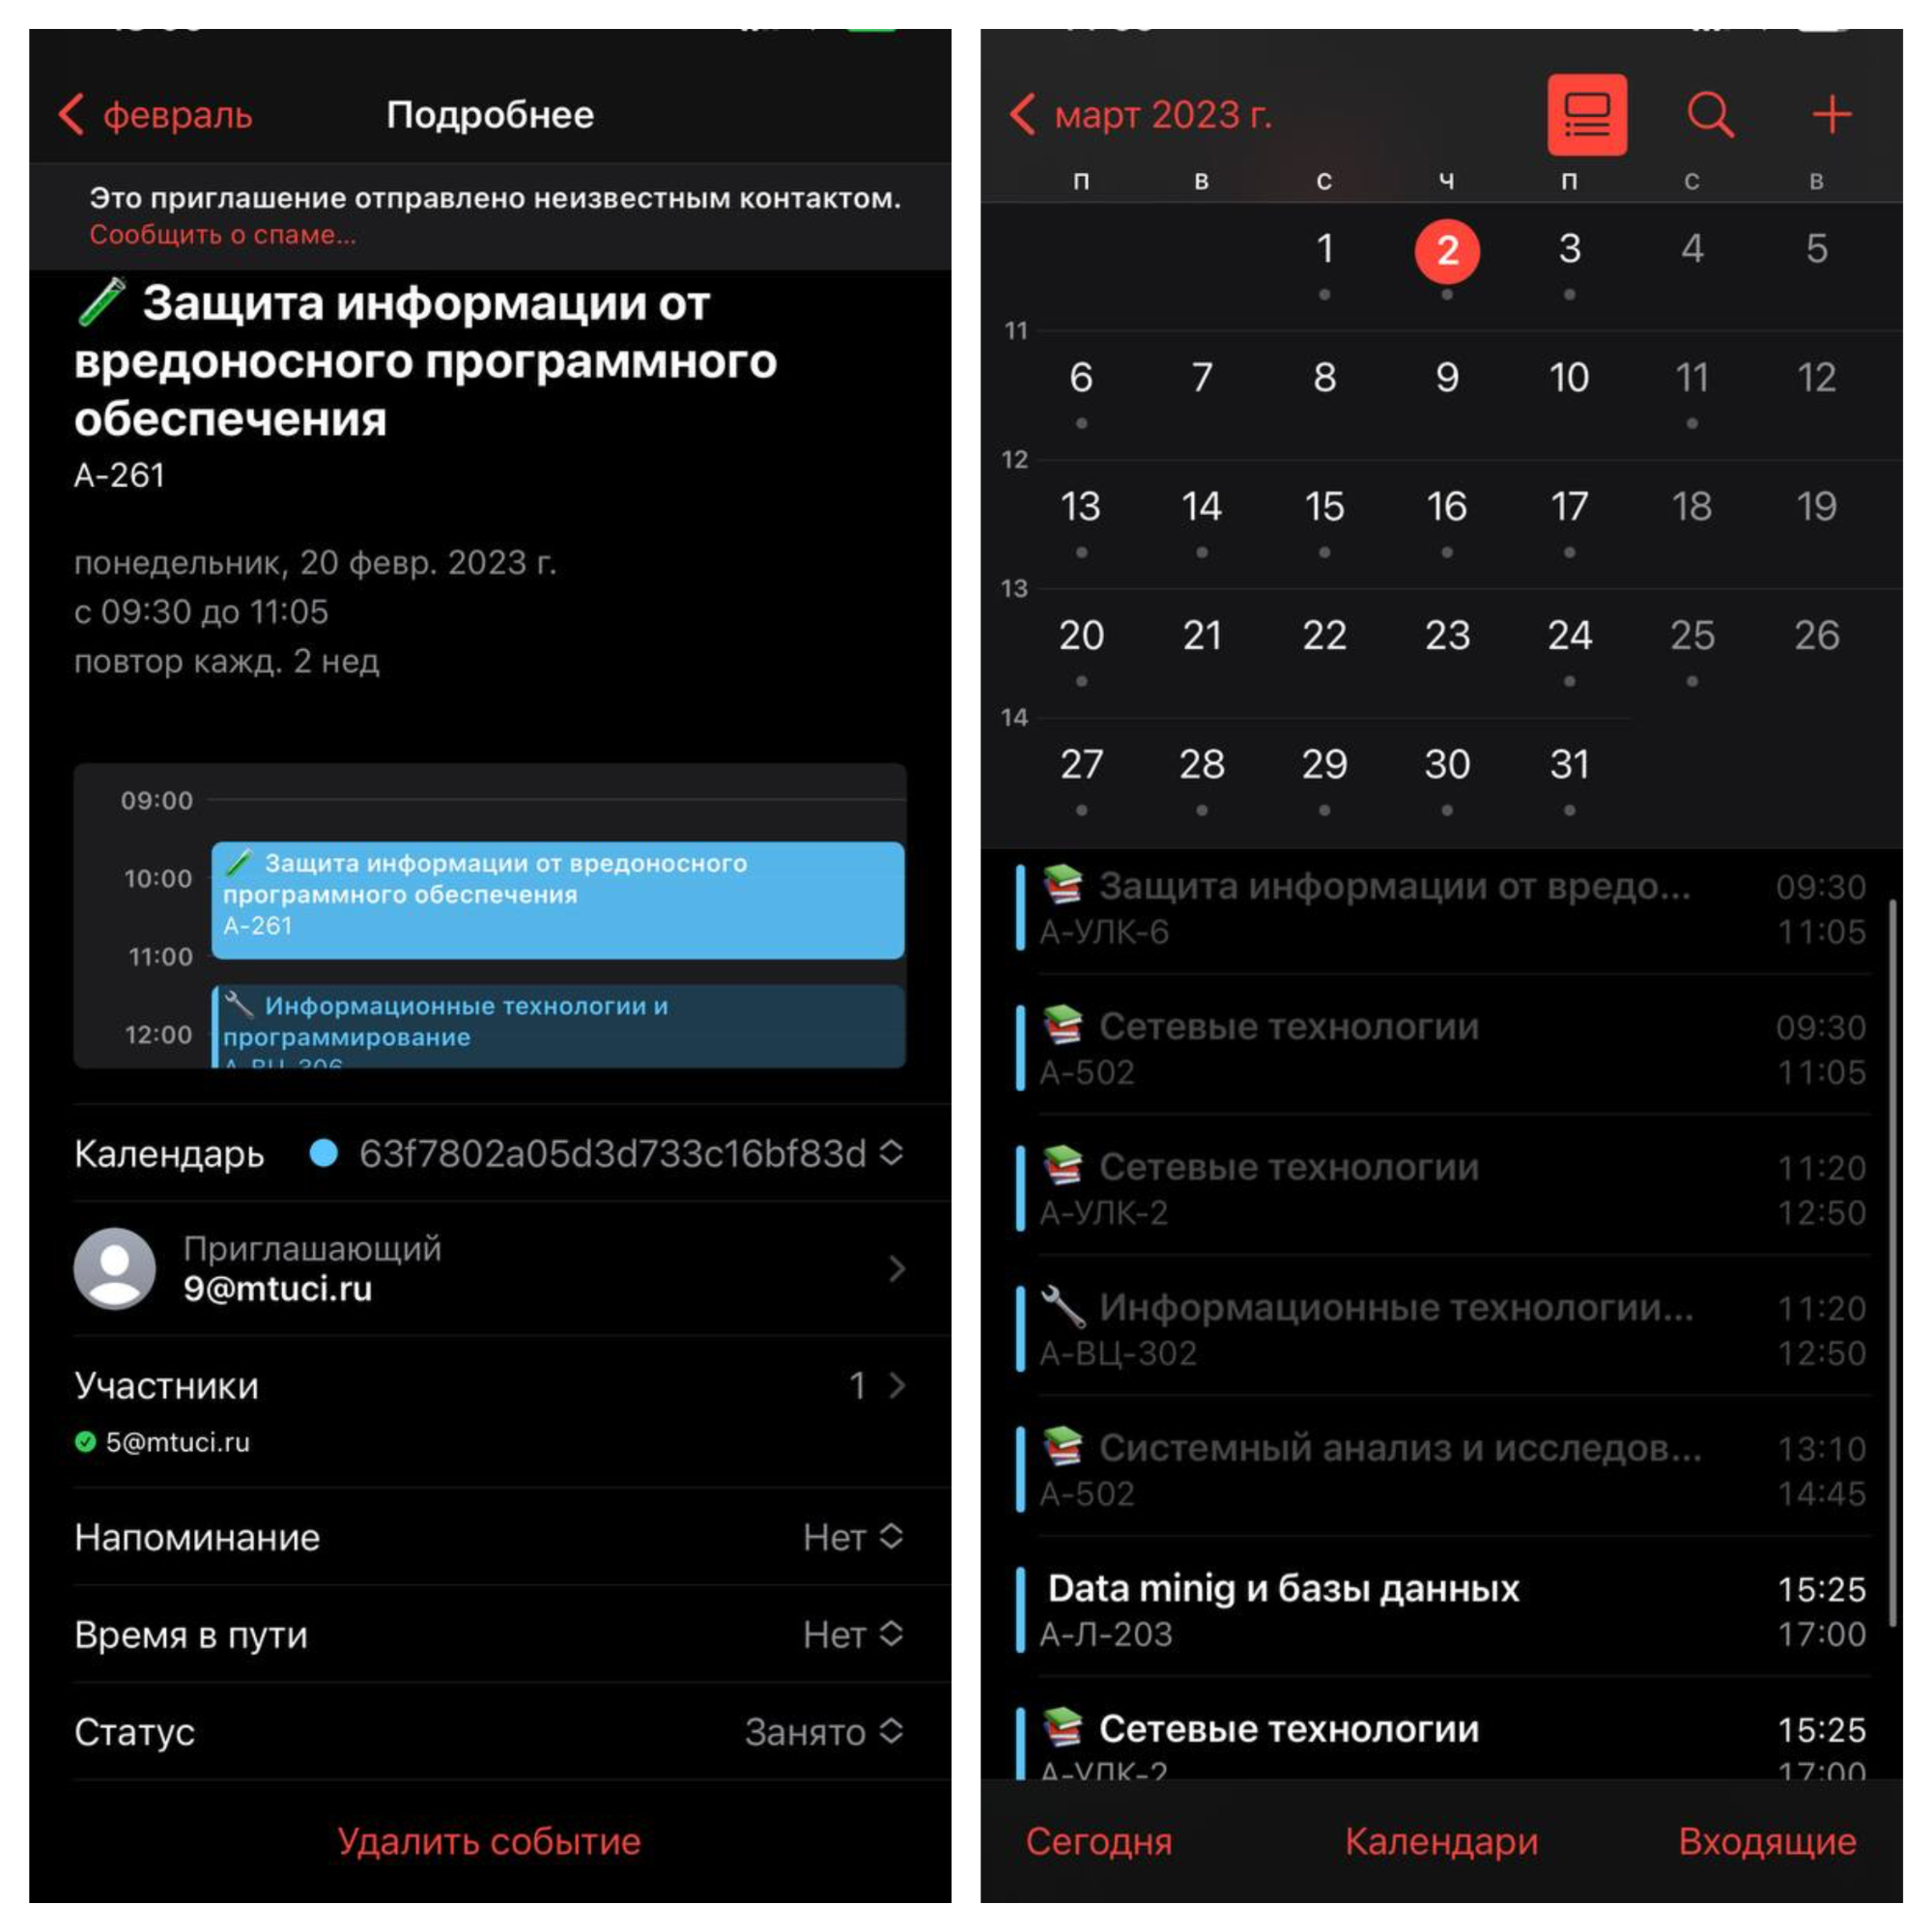
\includegraphics[width=0.7\linewidth]{images/back/ics.png}
  \caption{Пример отображения расписания занятий в iOS календаре}
  \label{fig:back:ics}
\end{figure}


На данный момент сервис активен, и его можно использовать по ссылке \url{http://mtuci.stereobreeze.ru/ics/*.ics}, 
где \texttt{*} - это ID фильтра, по которому будет сгенерирован ICS файл.
Исходный код сервиса расположен на доступен по ссылке \url{https://github.com/alexsvdk/mtuci_rasp_back/tree/master/ics_backend}.

\section{Процесс разработки мобильного приложения}
В процессе разработки мобильного приложения необходимо взаимодействовать с API backend-сервиса для получения данных расписания. 
Для этого используется HTTP-клиент Dio, который обеспечивает удобный способ отправки HTTP-запросов и обработки ответов. 
Dio поддерживает различные методы запросов (GET, POST, PUT, DELETE и другие) и позволяет работать 
с различными форматами данных, такими как JSON и XML.

В качестве управления состоянием приложения была выбрана библиотека riverpod. 
Riverpod обеспечивает удобную и декларативную модель управления состоянием, 
что помогает организовать эффективное взаимодействие с API и обновление пользовательского интерфейса приложения.

Процесс разработки мобильного приложения начинается с создания базовой структуры проекта. 
В качестве основного подхода к созданию структуры проекты был выбран feature first подход.
Каждый экран приложения представляет собой отдельный модуль,
который содержит в себе все необходимые для работы компоненты, такие как UI, логика и стейт-менеджмент.
Это позволяет разработчикам быстро ориентироваться в коде и упрощает процесс разработки и поддержки приложения.

Бузесовно, приложение содержит и код, которая используется на нескольких экранах сразу. Например дизайн, утилиты, модели данных и т.д.
Для такого кода был создан отдельный модуль, который содержит в себе все общие компоненты приложения.

Далее следует разработка пользовательского интерфейса (UI). 
Используя инструменты и виджеты, предоставляемые Flutter, удалось создать красивый 
и интуитивно понятный интерфейс для пользователей. 
Были учтены принципы хорошего дизайна пользовательского интерфейса, 
такие как ясность, доступность и согласованность. 

После разработки пользовательского интерфейса следует реализация логики приложения.
Здесь просиходит обработка взаимодействие пользователя с интерфейсом, обработка событий и валидация данных.
Для управления состоянием приложения можно использовать паттерн управления состоянием State Notifier, и реактивный подход.
View (экран) подписывается на изменения состояния и обновляет себя при изменении состояния.
Это поможет структурировать и упростить код, а также обеспечить эффективное управление состоянием приложения.

Для взаимодействия с сервисом backend мобильное приложение использует Graphql API,
предоставленное сервисом. С использованием HTTP-клиента Dio, приложение отправляет запросы к API,
получает ответы и обрабатывает полученные данные.

Для удобной работы с Graphql API была использована библиотека ferry, которая предоставляет удобный способ взаимодействия с API.
Для генерации кода запросов и моделей данных используется плагин ferry\textunderscore generator, который генерирует код на основе GraphQL схемы.
Это позволяет упростить процесс разработки и поддержки приложения, а также обеспечить безопасность типов при работе с данными.

По завершению разработки мобильного приложения, оно может быть развернуто на мобильных устройствах или платформах для публикации приложений, 
таких как Google Play Store или Apple App Store. При публикации необходимо обеспечить 
соответствие требованиям платформы и пройти процесс регистрации и публикации приложения.

В результате процесса разработки мобильного приложения будет получен готовый продукт, 
который позволит пользователям удобно и эффективно взаимодействовать с сервисом backend 
и получать актуальную информацию о расписании занятий.

\subsection{Экран поиска}
Экран поиска является одной из ключевых функций сервиса.
Он позволяет пользователям быстро находить расписания занятий и экзаменов по различным параметрам.
Скриншот экрана поиска представлен на рисунке \ref{fig:app:search}.

Пользователи могут искать информацию по:
\begin{enumerate}
    \item Группе
    \item Аудитории
    \item Преподавателю
    \item Предмету
\end{enumerate}

Подсказки отображаются на экране поиска в реальном времени, когда пользователь начинает вводить запрос.
Когда пользователь начинает вводить буквы, экран поиска предлагает список наиболее подходящих результатов,
основанных на уже введенных символах.
Например, если пользователь начинает вводить название группы,
экран поиска предлагает список всех групп, у которых в названии есть введенные символы.
Пользователь может выбрать нужную группу из списка и получить соответствующее расписание занятий и экзаменов.
Этот механизм упрощает поиск информации для пользователей.

На экране поиска есть кнопка "Добавить в календарь",
которая позволяет пользователям подписаться на календарь по URL
и получать обновленное расписание занятий и экзаменов
в своем календаре без необходимости ручного импорта файла.
Это реализовано при помощи микросервиса, который генерирует ICS-файл
на основе полученных данных и сохраняет его в файловое распределенное хранилище S3.
При последующих обращениях по URL микросервис проверяет актуальность
уже генерированного файла при помощи механизма ведения ревизий,
и если файл все еще актуальный - возвращает HTTP код переадресации на ICS из файлового хранилища.

\begin{figure}
\centering
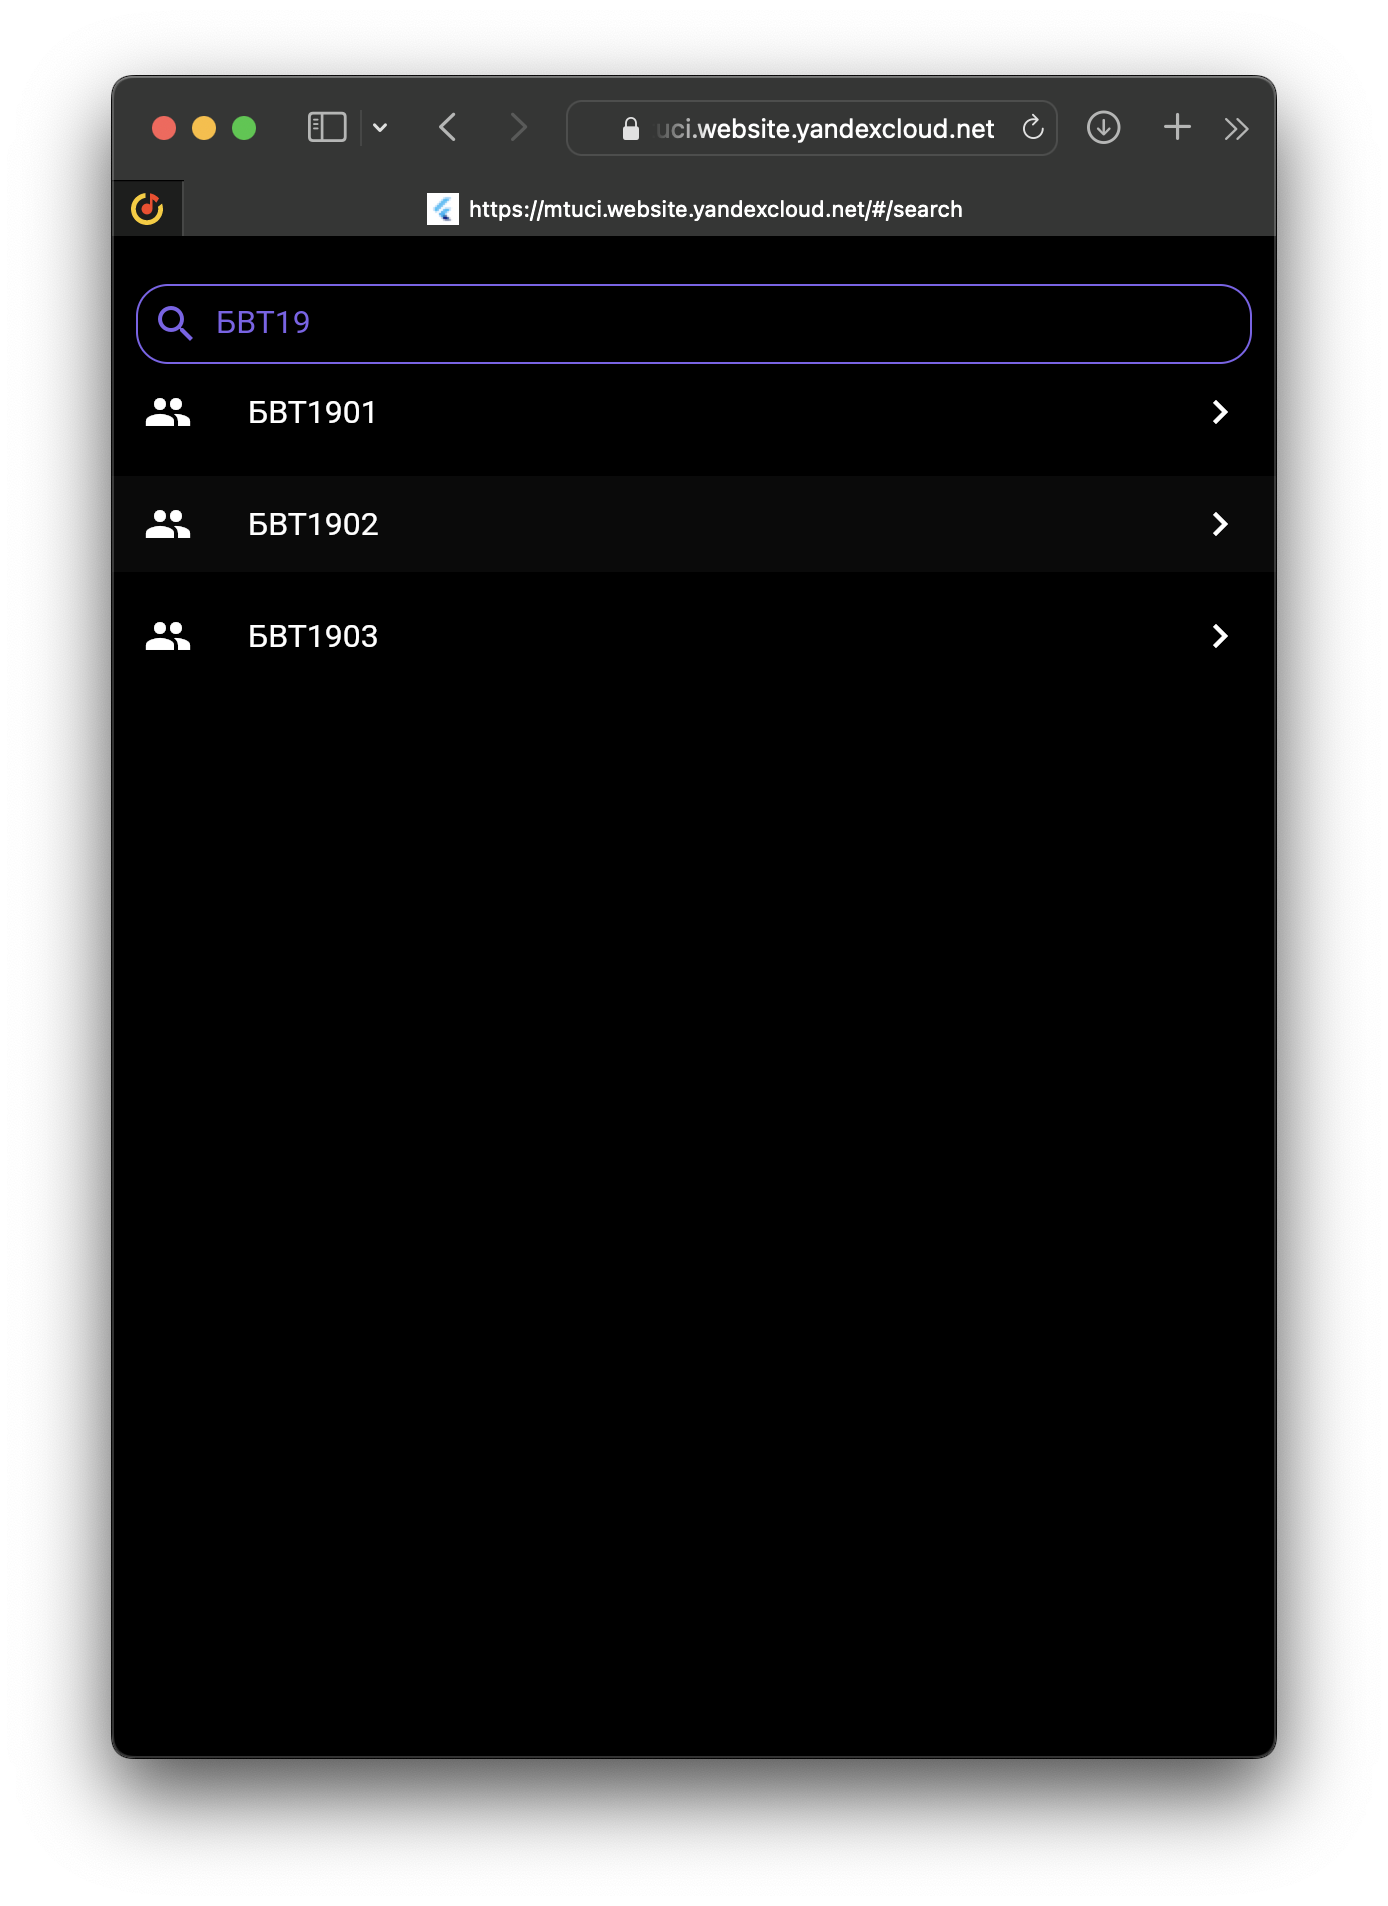
\includegraphics[width=0.7\linewidth]{images/app/search.png}
\caption{Скриншот экрана поиска}
\label{fig:app:search}
\end{figure}

\break
\subsection{Экран расписания}
Экран расписания является одним из ключевых элементов приложения для получения расписания МТУСИ.
На этом экране пользователи могут увидеть расписание занятий на конкретный день. 
Скриншот экрана расписания представлен на рисунке \ref{fig:app:rasp}.

Экран содержит следующие элементы:
\begin{enumerate}
    \item Возможность возврата к поиску, 
    чтобы пользователи могли быстро изменить параметры поиска и найти нужное расписание.
    \item Расписание занятий на конкретный день.
    Пользователи могут просмотреть расписание занятий для выбранной группы,
    преподавателя, аудитории или предмета на любую дату.
    \item Если на выбранный день нет занятий,
    то есть кнопка, которая ведет к ближайшим датам занятий.
    Пользователи могут увидеть, когда будут следующие занятия и планировать свое время соответственно.
\end{enumerate}


\begin{figure}
\centering
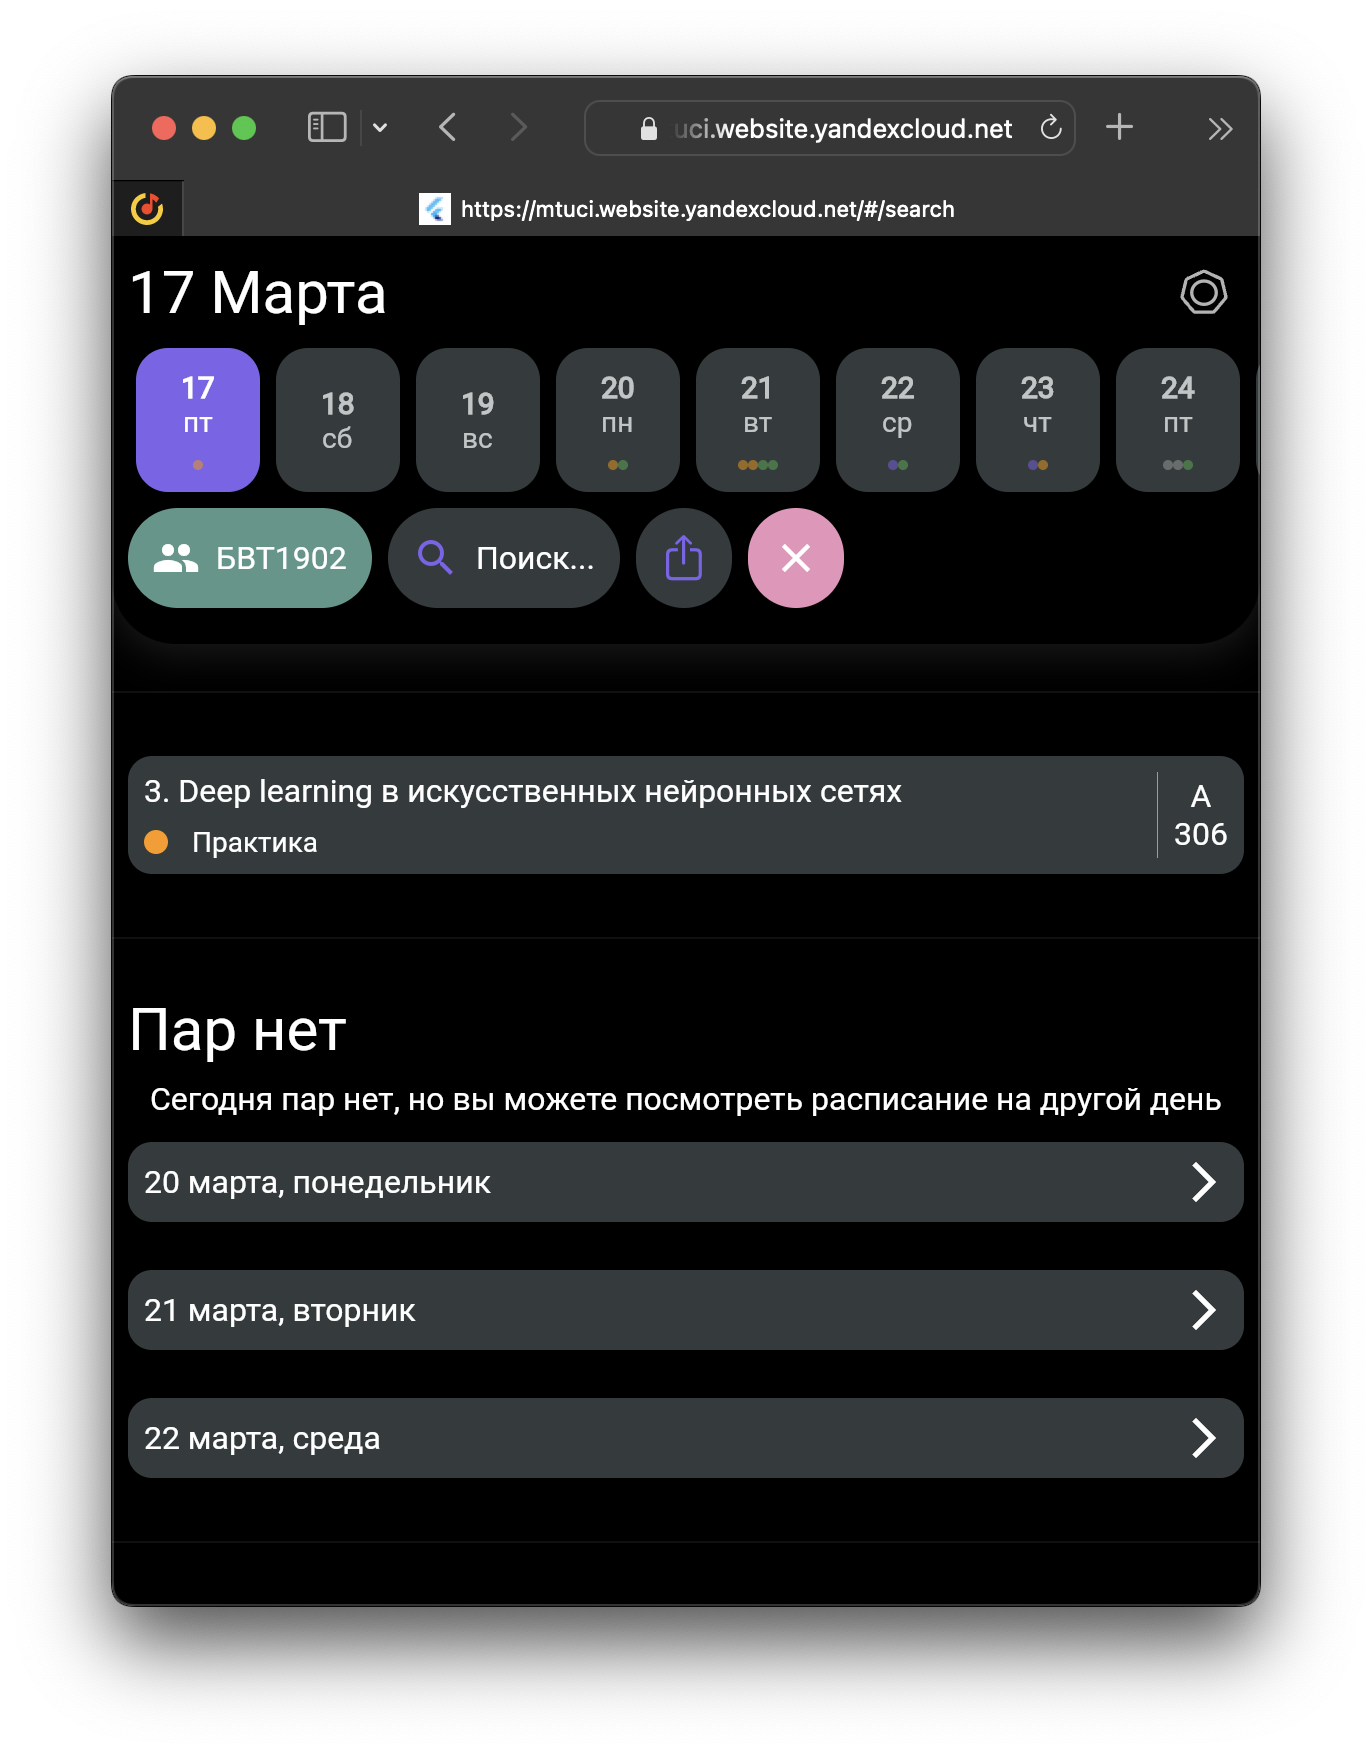
\includegraphics[width=0.5\linewidth]{images/app/rasp.png}
\caption{Скриншот экрана расписания}
\label{fig:app:rasp}
\end{figure}

В целом, экран расписания является важным элементом приложения
для получения расписания МТУСИ, который помогает пользователям оставаться
в курсе своих занятий и экзаменов.

\subsection{Экран настроек}
Экран настроек предоставляет пользователям возможность настроить
приложение на свой вкус и свои потребности.
Он содержит ряд настроек, которые помогают улучшить
пользовательский опыт и сделать использование приложения более комфортным.
Скриншот экрана настроек представлен на рисунке \ref{fig:app:settings}.

В приложении можно регулировать следующие настройки:
\begin{enumerate}
    \item Настройка \textbf{языка} приложения позволяет пользователям лучше понимать интерфейс и функциональность приложения.
    \item Экран настроек также позволяет выбрать \textbf{тему} приложения (темную или светлую),
    которая наиболее комфортна для глаз и соответствует условиям окружающей среды. 
    \item Наконец, пользователи могут отправить \textbf{сообщение разработчику} приложения,
    чтобы получить поддержку в случае необходимости.
\end{enumerate}

\begin{figure}
\centering
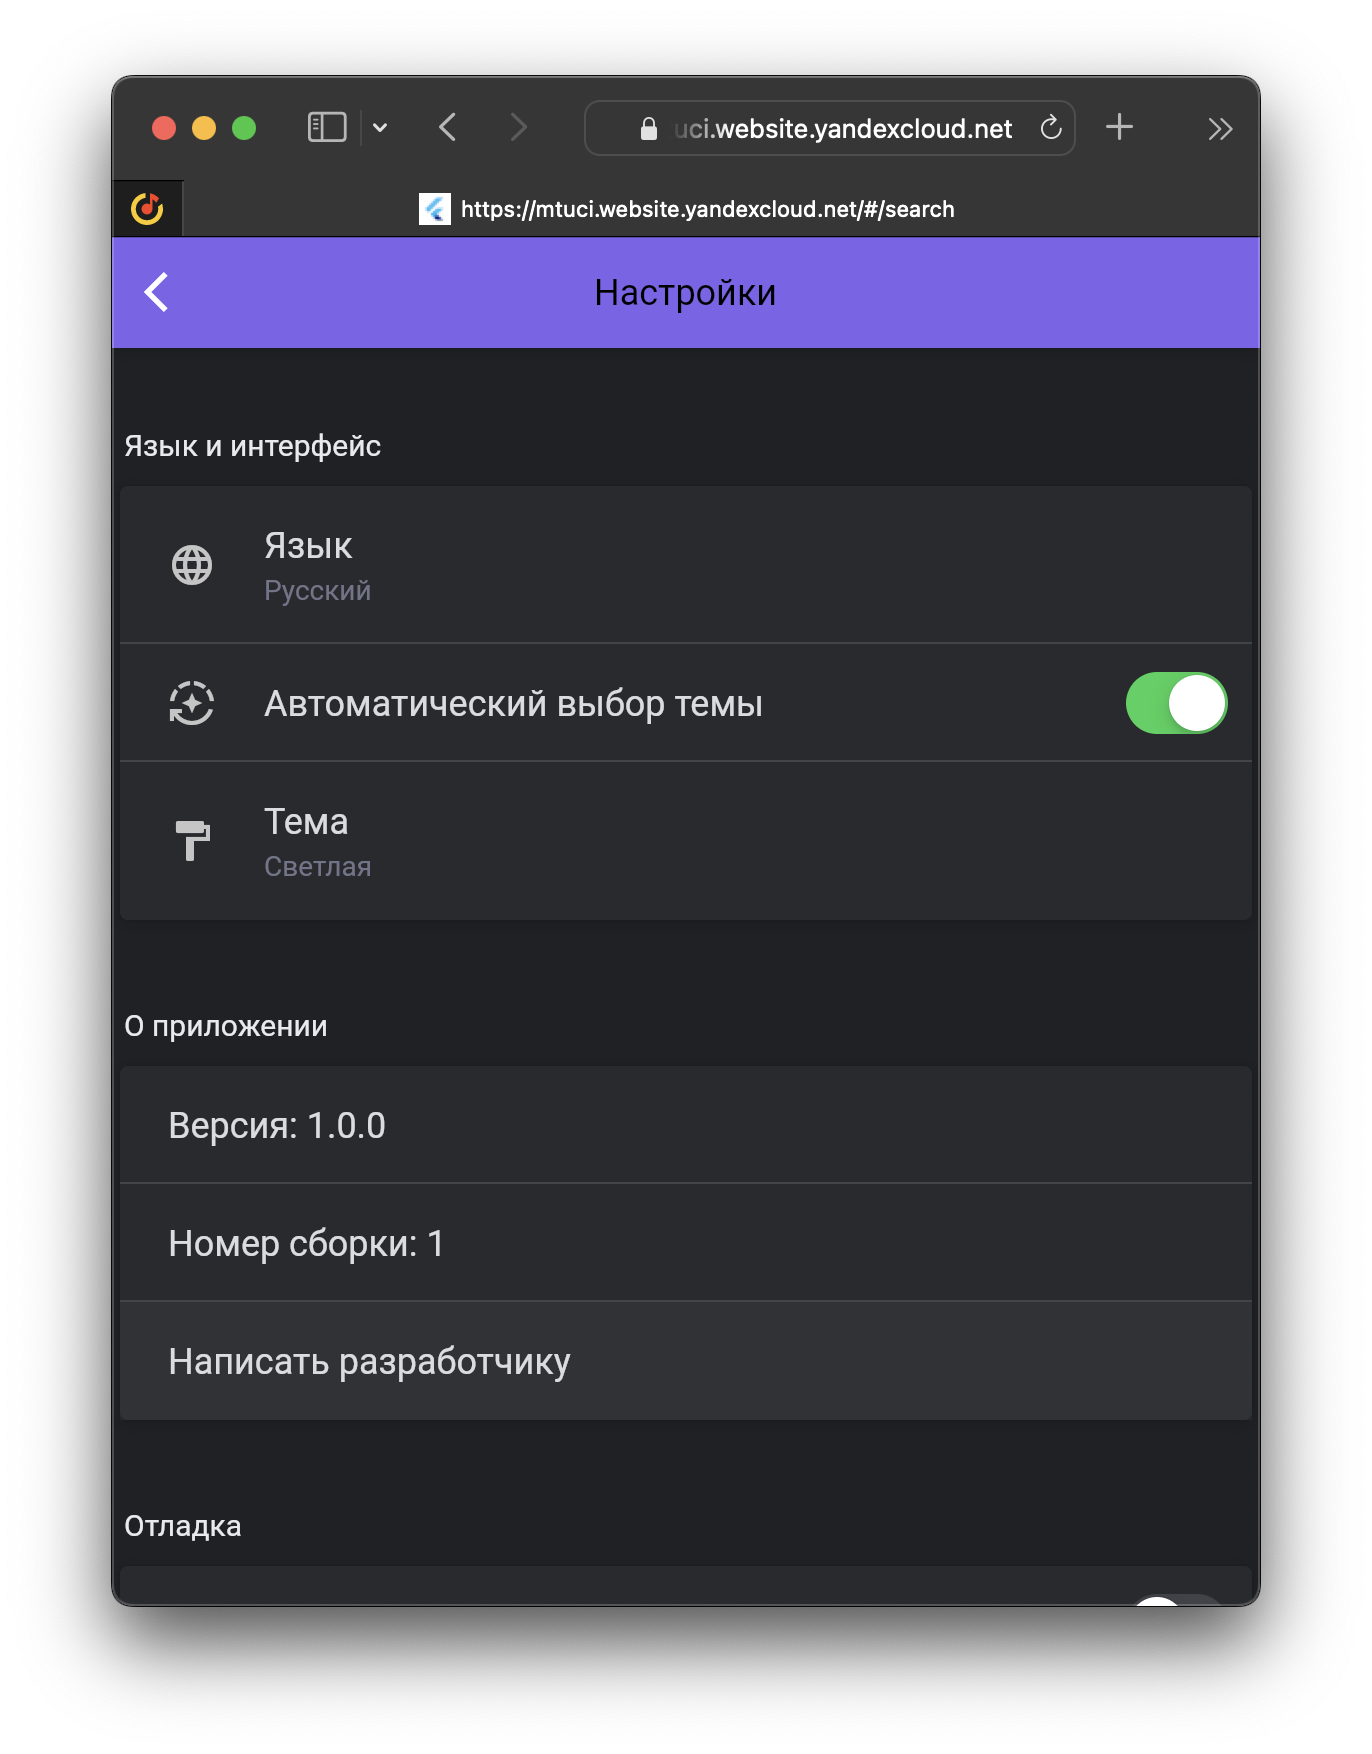
\includegraphics[width=0.5\linewidth]{images/app/settings.png}
\caption{Скриншот экрана настроек}
\label{fig:app:settings}
\end{figure}

В целом, экран настроек является важным элементом приложения,
который помогает пользователям настроить приложение на свой вкус и
решить любые вопросы, связанные с использованием приложения.

\break
\subsection{Экран одного занятия}
На экране одного занятия пользователи могут получить подробную информацию о конкретном занятии или экзамене.
Скриншот экрана одного занятия представлен на рисунке \ref{fig:app:lesson}.
Этот экран предоставляет детали занятия,
такие как:
\begin{enumerate}
    \item Дата
    \item Время
    \item Место проведения
    \item Название группы
    \item ФИО преподавателя
    \item Название предмета
\end{enumerate}

\begin{figure}
\centering
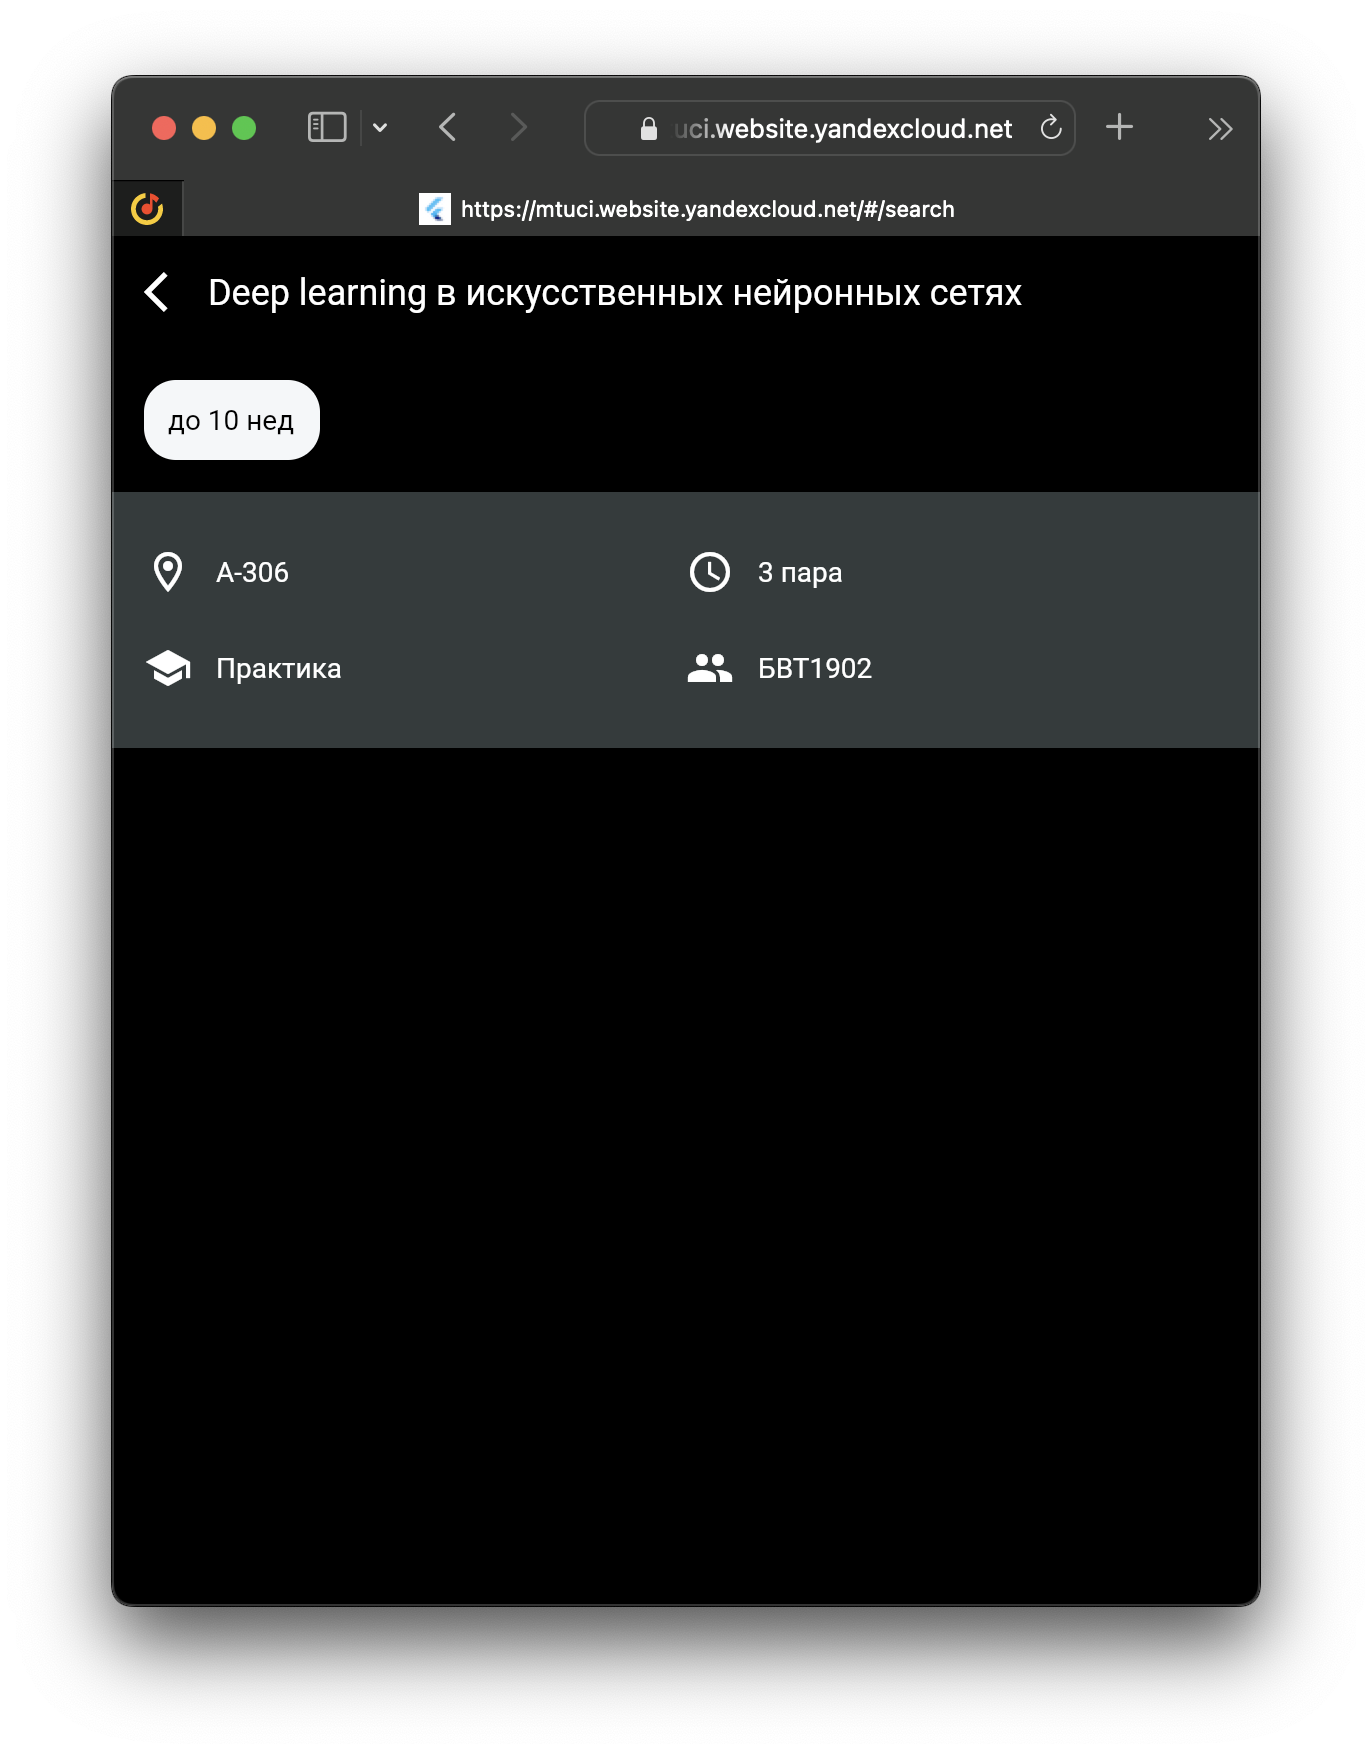
\includegraphics[width=0.5\linewidth]{images/app/lesson.png}
\caption{Скриншот экрана одного занятия}
\label{fig:app:lesson}
\end{figure}

Экран одного занятия является важным элементом приложения,
который помогает пользователям получать детальную информацию
о своих занятиях и планировать свое расписание соответственно.
Благодаря этому экрану, пользователи могут легко организовать
свое время и не пропускать важные занятия и экзамены.

\section{Кроссплатформенность}
Приложение разрабатывается с учетом кроссплатформенности и может быть запущено на различных платформах,
включая iOS, Android и веб-браузеры.
Для этого используются современные технологии разработки, такие как Flutter и GraphQL API.
Такой подход позволяет достичь максимальной доступности приложения для пользователей и обеспечить единый
интерфейс и функциональность на разных платформах.

\begin{enumerate}
    \item \textbf{WEB} - приложение доступно в браузерах, таких как Google Chrome, Mozilla Firefox и Safari. 
    Оно адаптировано для работы на смартфонах, и может быть добавлено на главный экран как PWA (Progressive Web App).
    На данный момент приложение доступно по адресу \url{https://mtuci.website.yandexcloud.net}.
    \item \textbf{Android} - приложение доступно для смартфонов и планшетов на базе операционной системы Android.
    На данный момент приложение можно загрузить по адресу \url{https://storage.yandexcloud.net/mtuci/app-release.apk}.
    \item \textbf{iOS} - приложение доступно для смартфонов и планшетов на базе операционной системы iOS.
\end{enumerate}

\section{Развертывание АИС}
Для развертывания АИС был выбран сервис Yandex Cloud, который предоставляет виртуальные машины 
с предустановленными операционными системами и другими компонентами, необходимыми для работы АИС.
Для развертывания АИС была выбрана операционная система Ubuntu 20.04 LTS, так как она является 
одной из самых популярных и поддерживаемых операционных систем в мире.
Ресурсы виртуальной машины были выбраны с учетом потенциальной нагрузки на АИС и составили:
\begin{enumerate}
    \item 4 vCPU
    \item 4 GB RAM
    \item 50 GB HDD
\end{enumerate}

Далее на виртуальной машине было установлено необходимое программное обеспечение, включая:
\begin{enumerate}
    \item \textbf{Docker} - для развертывания и управления контейнерами.
    \item \textbf{Docker Compose} - для развертывания и управления многоконтейнерными приложениями.
    \item \textbf{JDK} - для компиляции и запуска Java приложений.
    \item \textbf{MongoDB} - для хранения данных.
\end{enumerate}

После установки ПО следует был сконфигурирован каждый компонент АИС, 
включая сервис API, парсер расписания и ICS API. 
Это включает настройку соединения с базой данных, 
настройку маршрутов и точек доступа для API, 
а также конфигурацию различных параметров и настроек.

Для внешнего доступа к АИС были открыты порты 80 и 443,
настроен nginx для проксирования запросов на сервис API и ICS API,
а также настроен SSL сертификат для обеспечения безопасного соединения.

Далее сислема была протестирована на работоспособность и было убеждено,
что все компоненты работают корректно и без ошибок.